%Para empezar, léete lo que he dicho de los otros capítulos - JJ FERGU: Cambiado el titulo
\myChapter{Development of a Service Oriented Architecture for Evolutionary Algorithms}\label{chap:osgiliath}
% Dedicar un capítulo a la implementación es arriesgado, porque una
% implementación no es parte de una tesis, es, bueno,
% implementación. Salvo que justifiques que realmente lo es,
% justifiques las elecciones hechas, deduzcas conclusiones generales,
% presentes una metodología (lo del SOMA ese), en principio, es dudoso
% que necesite un capítulo o incluso que vaya fuera de un apéndice - JJ

%FERGUSON: REESCRITO casi entero para seguir la metodología y borradas un porrón de cosas

%TODO:
% Quitar los "Could be"
\minitoc\mtcskip
\vfill
\lettrine{I}{n} Chapter \ref{chap:soaea} %we presented the services
%that conform an Evolutionary Algorithm  % ¿así, en general? ¿En qué
                                % contexto? - JJ
%and the process to design a service oriented EA. Although the previous
%examples can be developed using any SOA technology, this chapter
%presents OSGiLiath ({\em OSGi Laboratory for Implementation and
%  Testing of metaHeuristics}), an implementation of SOA-EA based in
%OSGi. % lo que hacemos porque... - JJ FERGUSON: comentado todo

IMPORTANTE: Decir que otra de las cosas que ofrece SOA es el auto-descubrimiento de servicios (Y LUEGO USARLO EN EL CAPITULO DE HOMOHETERO)

Previous chapter has presented a methodology to develop SOEAs. This chapter justifies the use of SOA-EA and the steps to create services within it. Solving the questions in each step leads to...

Then, for the implementation and deployment step, we will use a specific SOA technology (OSGi) to implement and deploy all the examples shown in previous sections, and how to accomplish the requirements in the development of EAs and SOA, taking advantage of the capabilities of SOA. As this is an iterative and and incremental methodology, new services can be discovered or removed in next steps (for example, infrastructure services).

\section{Example of creating a service oriented evolutionary algorithm}
\label{sec:soaea:creating}
 
In this example a basic Service Oriented Genetic Algorithm is designed. Then, to illustrate the iterative process of the proposed methodology and the capabilities of using SOA, a NSGA-II algorithm is also designed using the existent services and adding new ones. Finally, new services for 

\subsection{Identification}
As  stated in in Section \ref{sec:distributed:types}, a basic EA is formed by several steps. Solving the questions in Section \ref{subsec:soaea:identification} and the considerations about the design of services (Section \ref{sec:soa:restrictions}) and the genericity of EAs (Section \ref{sec:distributed:design}) a number of abstract services have been identified. In the {\em algorithm domain}, the Algorithm, Population, Parent Selector, Recombinator, Mutator, Replacer, Stop Criterion and Parameters. In the {\em problem domain}, the Fitness Calculator and Initializer. %Finally, a {\em infrastructure domain} service called Asynchronous Enabler, which is in charge of activating new operators when a local optimum is found (for example, no changes in best individual during certain time). FERGU: mover esto al ejemplo de Enabler



\begin{itemize}
\item Algorithm
\item Population
\item Initializer
\item Parent Selector
\item Recombinator
\item Crossover
\item Mutator
\item Mutation
\item Replacer
\item Stop Criterion
\item Fitness Calculator
\item Parameters
\end{itemize}

\subsection{Specification}

 Concrete implementations are defined: {\em N Tournament} and {\em Roulette} are implementations of parent selectors and {\em Optimum Found} the desired stop criterion. Also, to address the problem to be solved, such as {\em MMDP Fitness Calculator} or {\em Binary Initializer}. As we need a fixed set of steps, a {\em Evolutionary Algorithm} service is created to model the flow of services. The discovered services have been specified to accept  a list of individuals. A service to gather all selectors in the environment is used.

  

\begin{itemize}
\item Basic Order
\item Random Mutation
\item NWorst individual replacer
\end{itemize}

\begin{SCfigure}[20][htb]
\centering
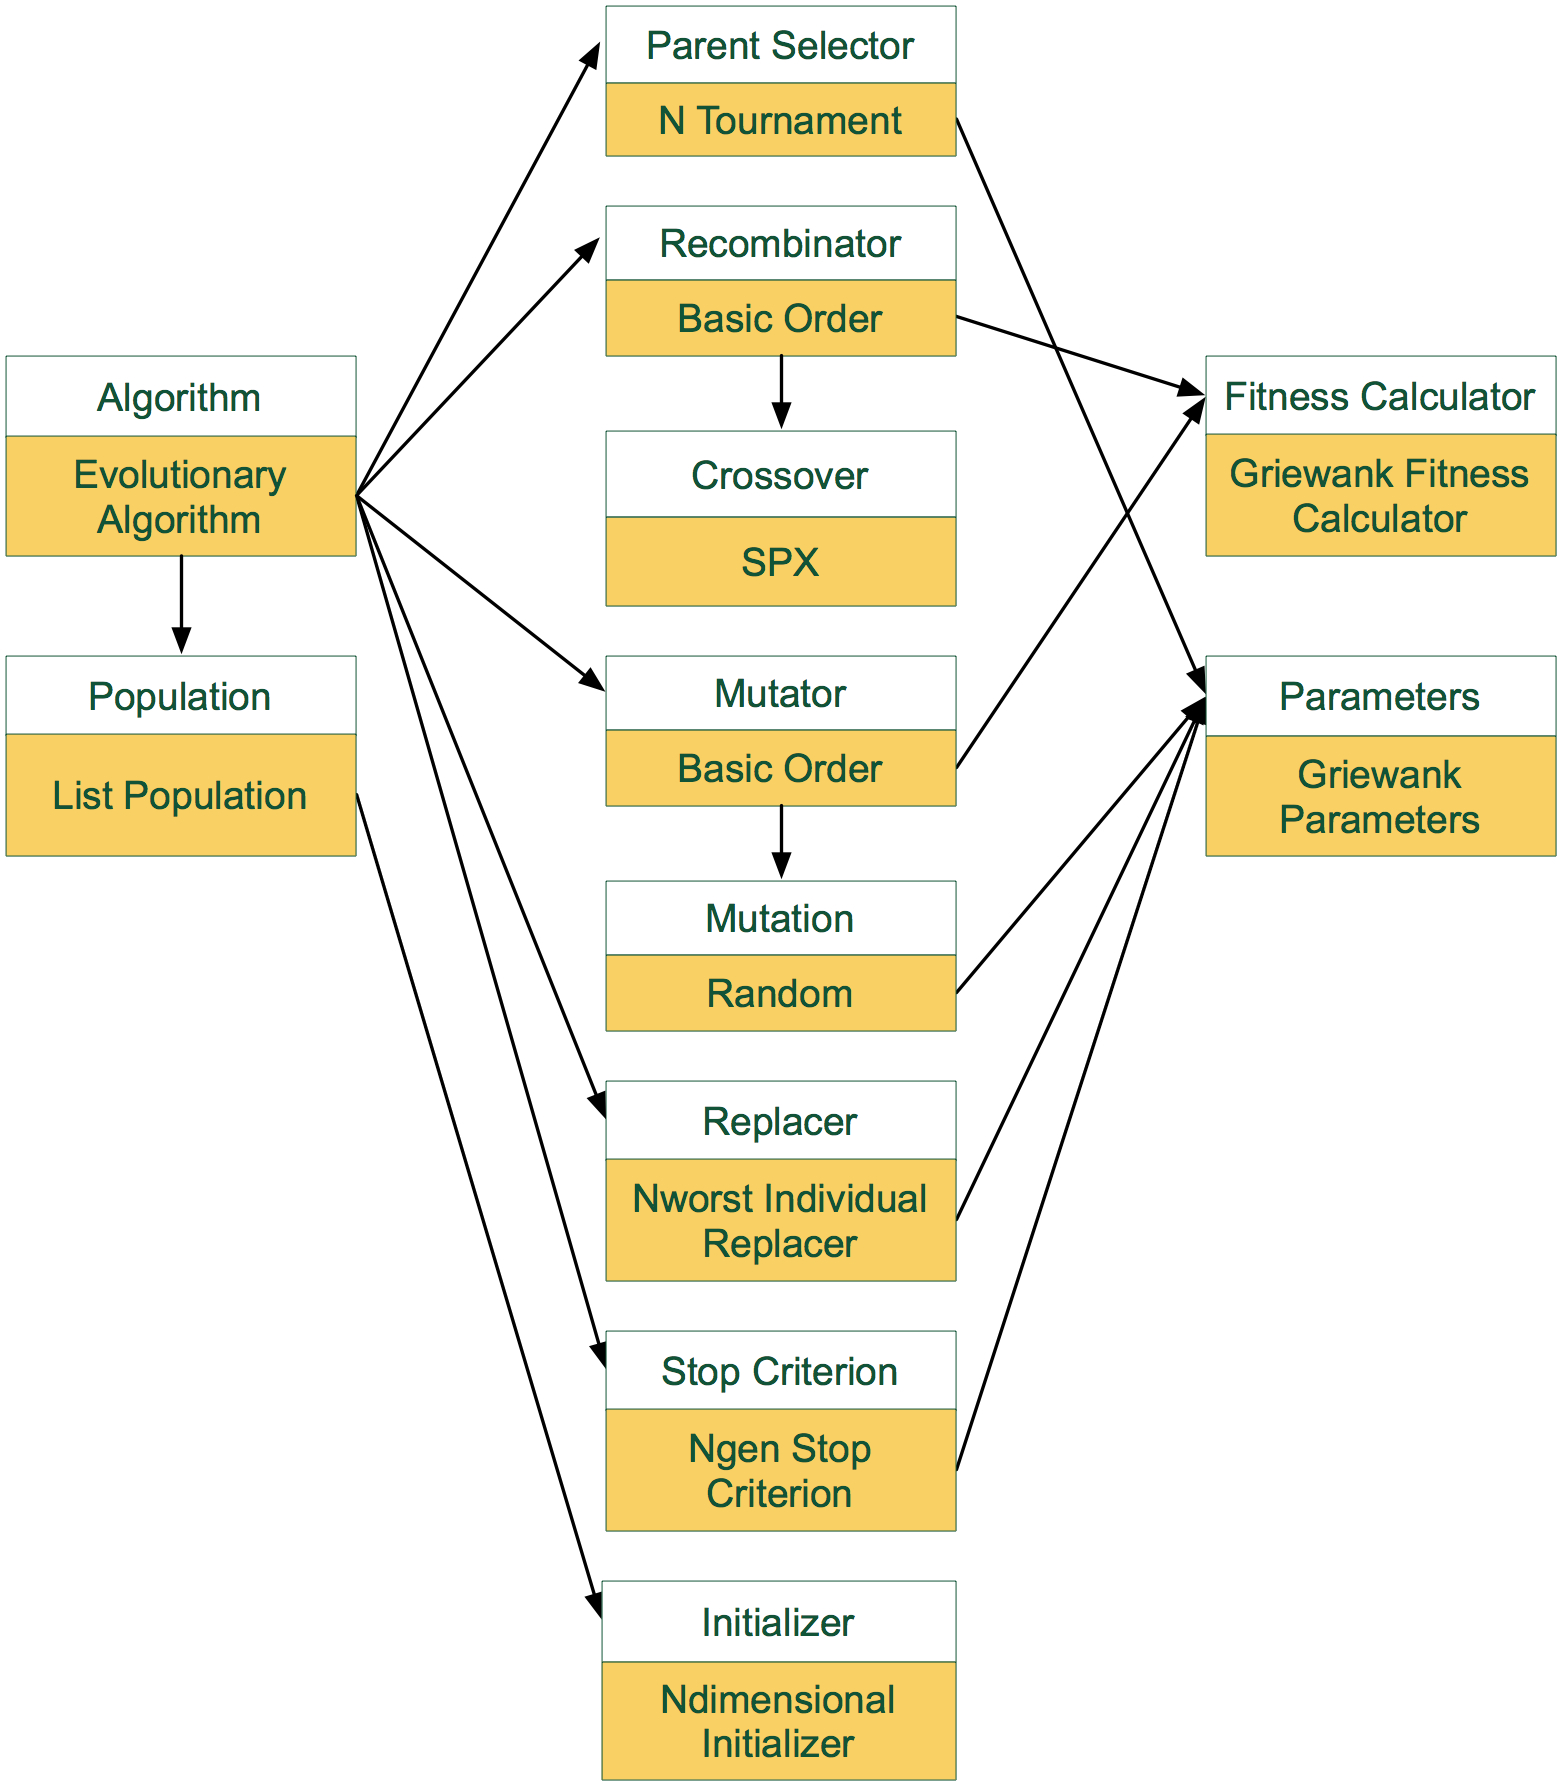
\includegraphics[width=10cm]{gfx/soaea/basicga.jpg}
\caption{Diagram of a basic genetic algorithm. White blocks are interfaces and orange blocks are implementations. In this case, we are using specific implementations to solve the OneMax problem.}
\label{BASICGAEXAMPLE}
\end{SCfigure}





Figure \ref{BASICGAEXAMPLE} shows the diagram of a complete service oriented genetic algorithm, taking into account the proposed ideas. In this figure (and in the following ones) white blocks are the service interfaces. Orange blocks are specific implementations of these interfaces (that is, the source-code of the service), and  arrows indicate how a service implementation can make use of other services via their interface. For example, almost all implementations access to the {\em Parameters} service using its interface. Service implementations (orange blocks) can be selected in a configuration file or be automatically bound when they are available (among other options).



 The change from a problem instance to another is quite simple. It is only necessary to notify the algorithm a change in the implementation of the service {\em Fitness Calculator}. Because some algorithms need to calculate the fitness every time an individual is modified (and not only at the end of a generation) the service {\em Fitness Calculator} may be used inside the implementations that modify individuals ({\em Initializer}, {\em Mutator} or {\em Recombinator}). Moreover, each service can be in the local machine or distributed on the Internet, having the same behaviour. %FERGU: TODO Decir que el fitness se usa solo si hace falta! Arreglado

\subsection{Extending the example to create a NSGA-II}
%\label{sec:nsga2}

As this is a iterative and incremental approach, other services can be discovered and designed in this step. For example, the difference between the previous version of a GA and the well known NSGA-II \cite{NSGA2} lies in the selection operator. Therefore, to change from the basic GA to NSGA-II, the mutator and crossover are kept and new selection operators are added. Figure \ref{fig:nsga2} shows the diagram of the service oriented version of NSGA-II algorithm, where the new implementations are marked with a thick border. The problem has also been changed to Multi-Objective Knacksack problem \cite{MULTIOBJECTIVEKNACKSACK}. New auxiliary services have been added, like {\em Crowding Distance Assignator} or {\em Pareto Assignator}. As these services may be used in other algorithms in the future, they should be designed as abstract as possible. These new services are called from the implementation (code) of the services {\em NSGA-II Replacer} or {\em Binary Crowding Distance Selector} (black arrows indicate an interface call). 




\begin{SCfigure}[20][htb]
\centering
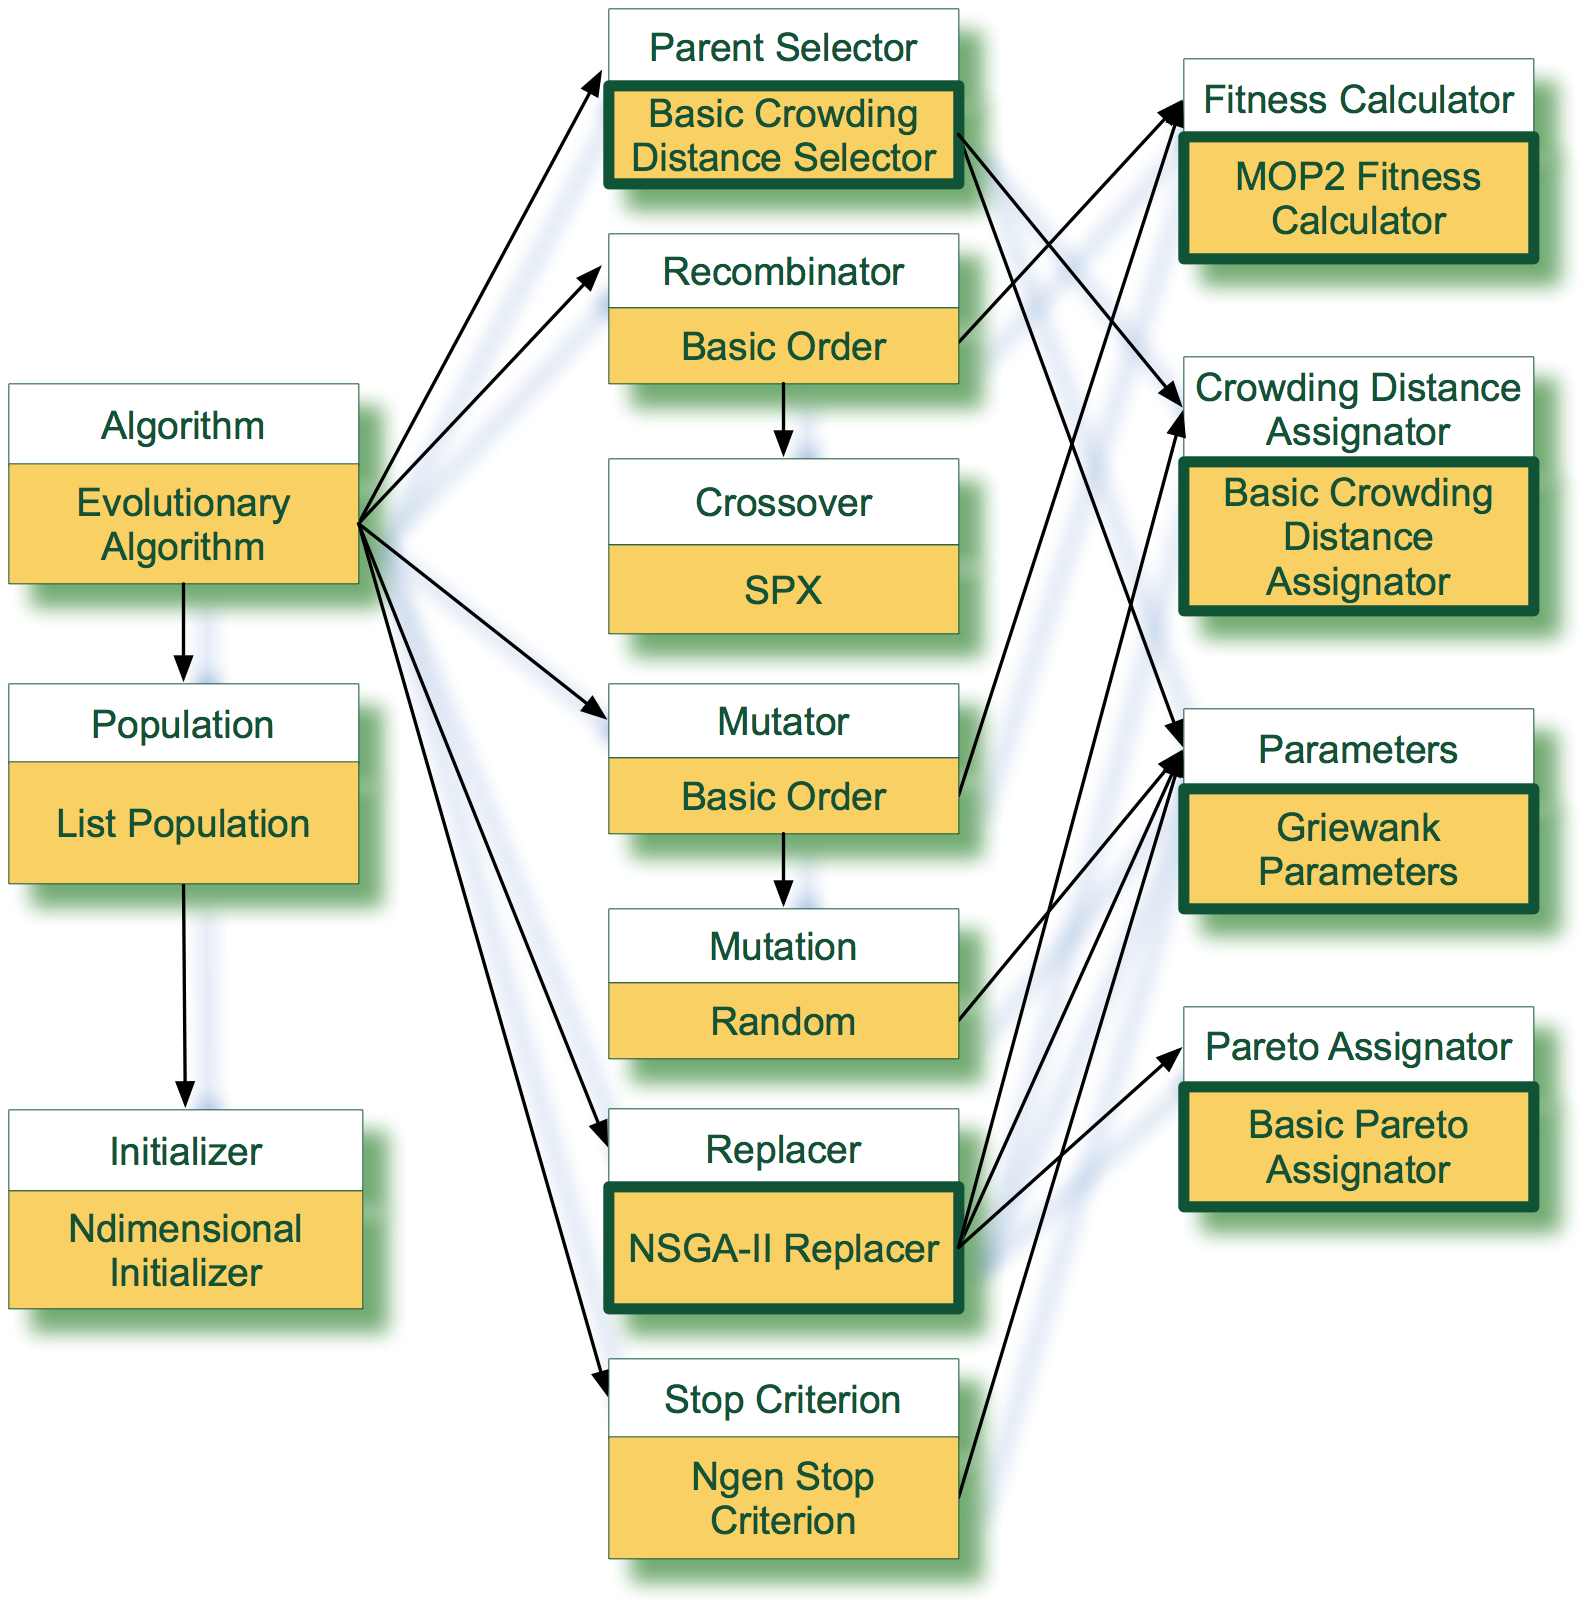
\includegraphics[width=10cm]{gfx/soaea/nsga2.jpg}
\caption{Modification of the basic GA adding new service implementations (orange blocks with thick lines).}
\label{fig:nsga2}
\end{SCfigure}



\subsection{Extending the example to add distribution}
\label{sec:distribution}

As every service must keep the same behaviour, independently of the machine that hosts it, distribution services for load balancing of a specific service can be easily created, for example, notifying the algorithm to use a distributed implementation for that service. As previously stated, the service {\em Fitness Calculator} receives a list of individuals to calculate their fitness, so, in this example, the new fitness implementation ({\em Basic Fitness Distributor}) binds with every fitness service available (in the same machine or in a network). The source code of this basic implementation simply distributes the list of individuals among the bound services and waits for their termination. Although more complex implementations probably will be more efficient, the objective of this section is to show how to distribute services, thus, this basic implementation is sufficient. Figure \ref{FITNESSDISTRIBUTOR} shows the modification from a sequential fitness calculator to a distributed one. Thanks to SOA, the number of distributed fitness calculators is not fixed: calculators can be added o removed in real time without stopping the system. As can be see in the figure, if one of the nodes is a cluster, it could also  implement another fitness distributor. This easy example can be adapted to more complex necessities depending on the infrastructure or the problem to be solved. More complex distribution services can be created, for example, taking into account communication latencies or computation capabilities of the nodes.




\begin{SCfigure}[20][htb]
\centering
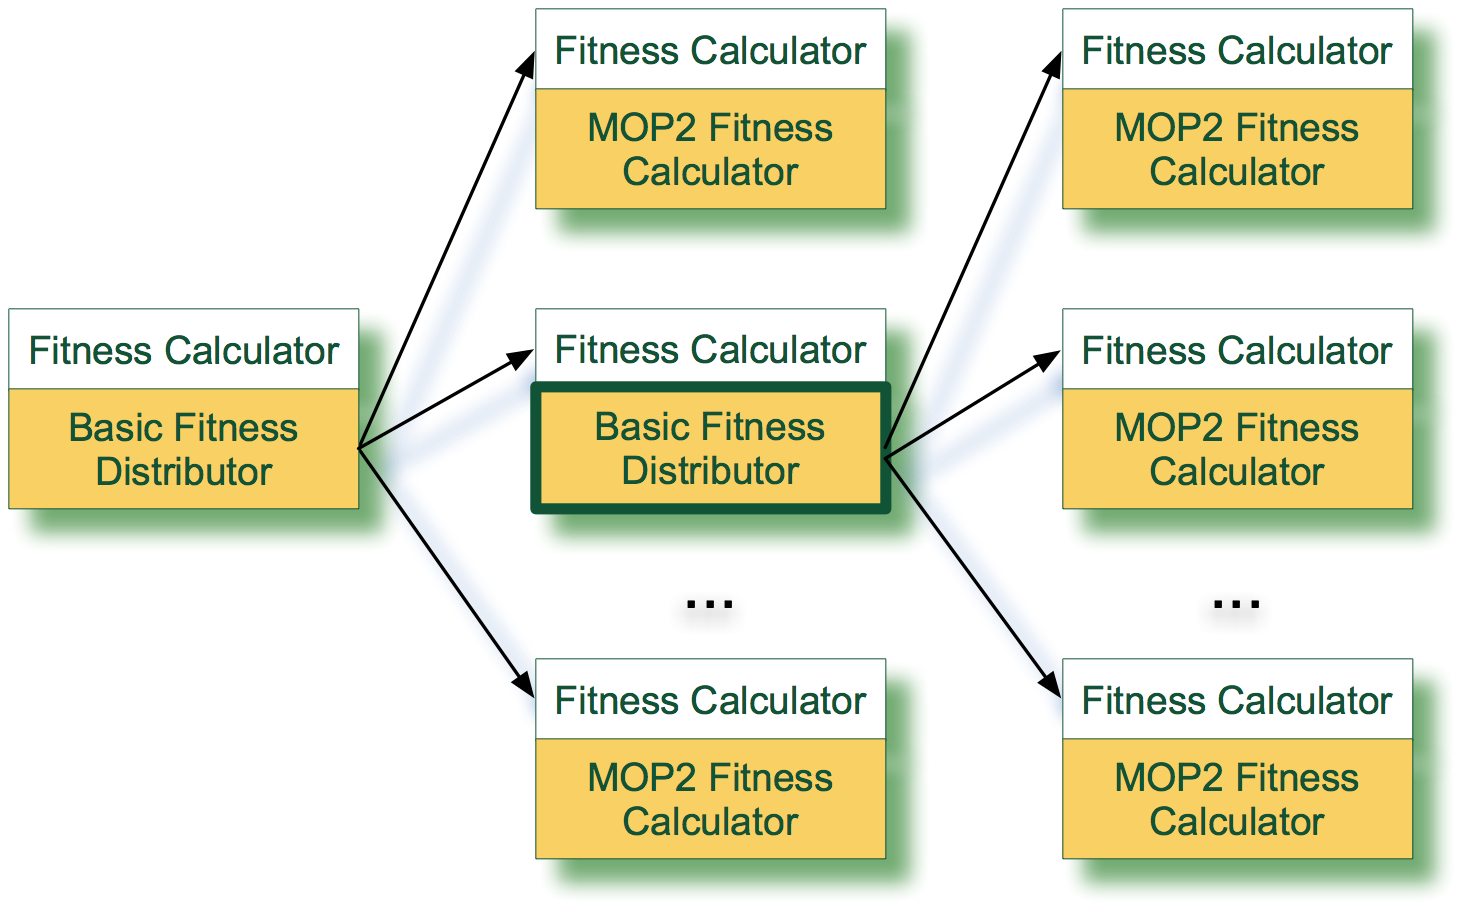
\includegraphics[width=10cm]{gfx/soaea/distributor.jpg}
\caption{Fitness distributor. The thick line implementation also re-distribute the individuals.}
\label{FITNESSDISTRIBUTOR}
\end{SCfigure}



One of the most extended model in parallel EAs is the island model. Using SOA-EA, the {\em Population} service implementation can be modified to become a distributed population. Each certain time, this population could exchange individuals with other populations modified by other algorithms. These populations should be added or deleted in execution time without affecting the algorithm execution. Figure \ref{POPULATION} shows this example, where a {\em Replacer} implementation maintains a list of references to other {\em Population} interfaces (which can be local or remote). Also other {\em Population} implementations exist ({\em List Population} is the usual list of individuals). If one of these population services drop, the others can continue working. The topology of these islands can also be managed from services (such as {\em Basic Replacer} service, or another). The  modification and dynamism of the population structure is difficult to apply in existing frameworks without using SOA because it is necessary to create mechanisms to modify the population behaviour, the operators to modify it, the data structures, and also the code to manage all. With he usage of SOA, and due to the capability of accessing to a population via its service interface, it is not necessary to modify the source code to modify the population and its behaviour. Also, to avoid bottlenecks in distributed executions, asynchronous communication must be provided to avoid idle time. This kind of communication offers excellent performance when working with different nodes and operating systems, as demonstrated by \cite{Alba2002Heterogeneous}.



\begin{SCfigure}[20][htb]
\centering
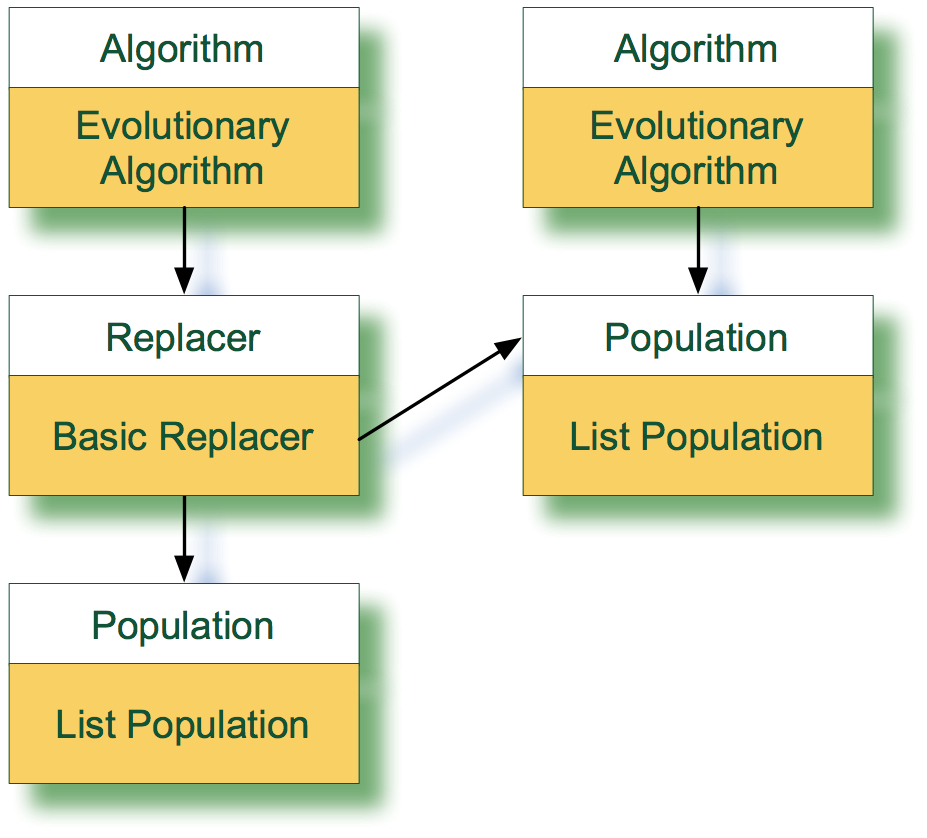
\includegraphics[width=7cm]{gfx/soaea/island.jpg}
\caption{Island model. From time to time, the Basic Replacer Implementation could send or receive individuals from other islands.}
\label{POPULATION}
\end{SCfigure}



\subsection{Self-adaptation of the services}
\label{sec:otherexamples}
There are several ways to create self-adaptable algorithms using SOA. For example, creating a service that modifies the parameters in the {\em Parameters} service, or activating and de-activating operators in real time. An easier way is to create a service that manages all available services of the same kind. For example a {\em Mutator} service that binds all the available mutation implementations and use the most adequate one depending on some rules during the execution \cite{SelfadaptationSerpell2010}.  This idea can also be extended to create a service that implements several interfaces and selects the most adequate implementation for each interface respect to some criteria, as can be seen in Figure \ref{INTELLIGENTALGORITHM}, where thick lines represent the implementations used at the current moment (they vary as time passes).



\begin{SCfigure}[20][htb]
\centering
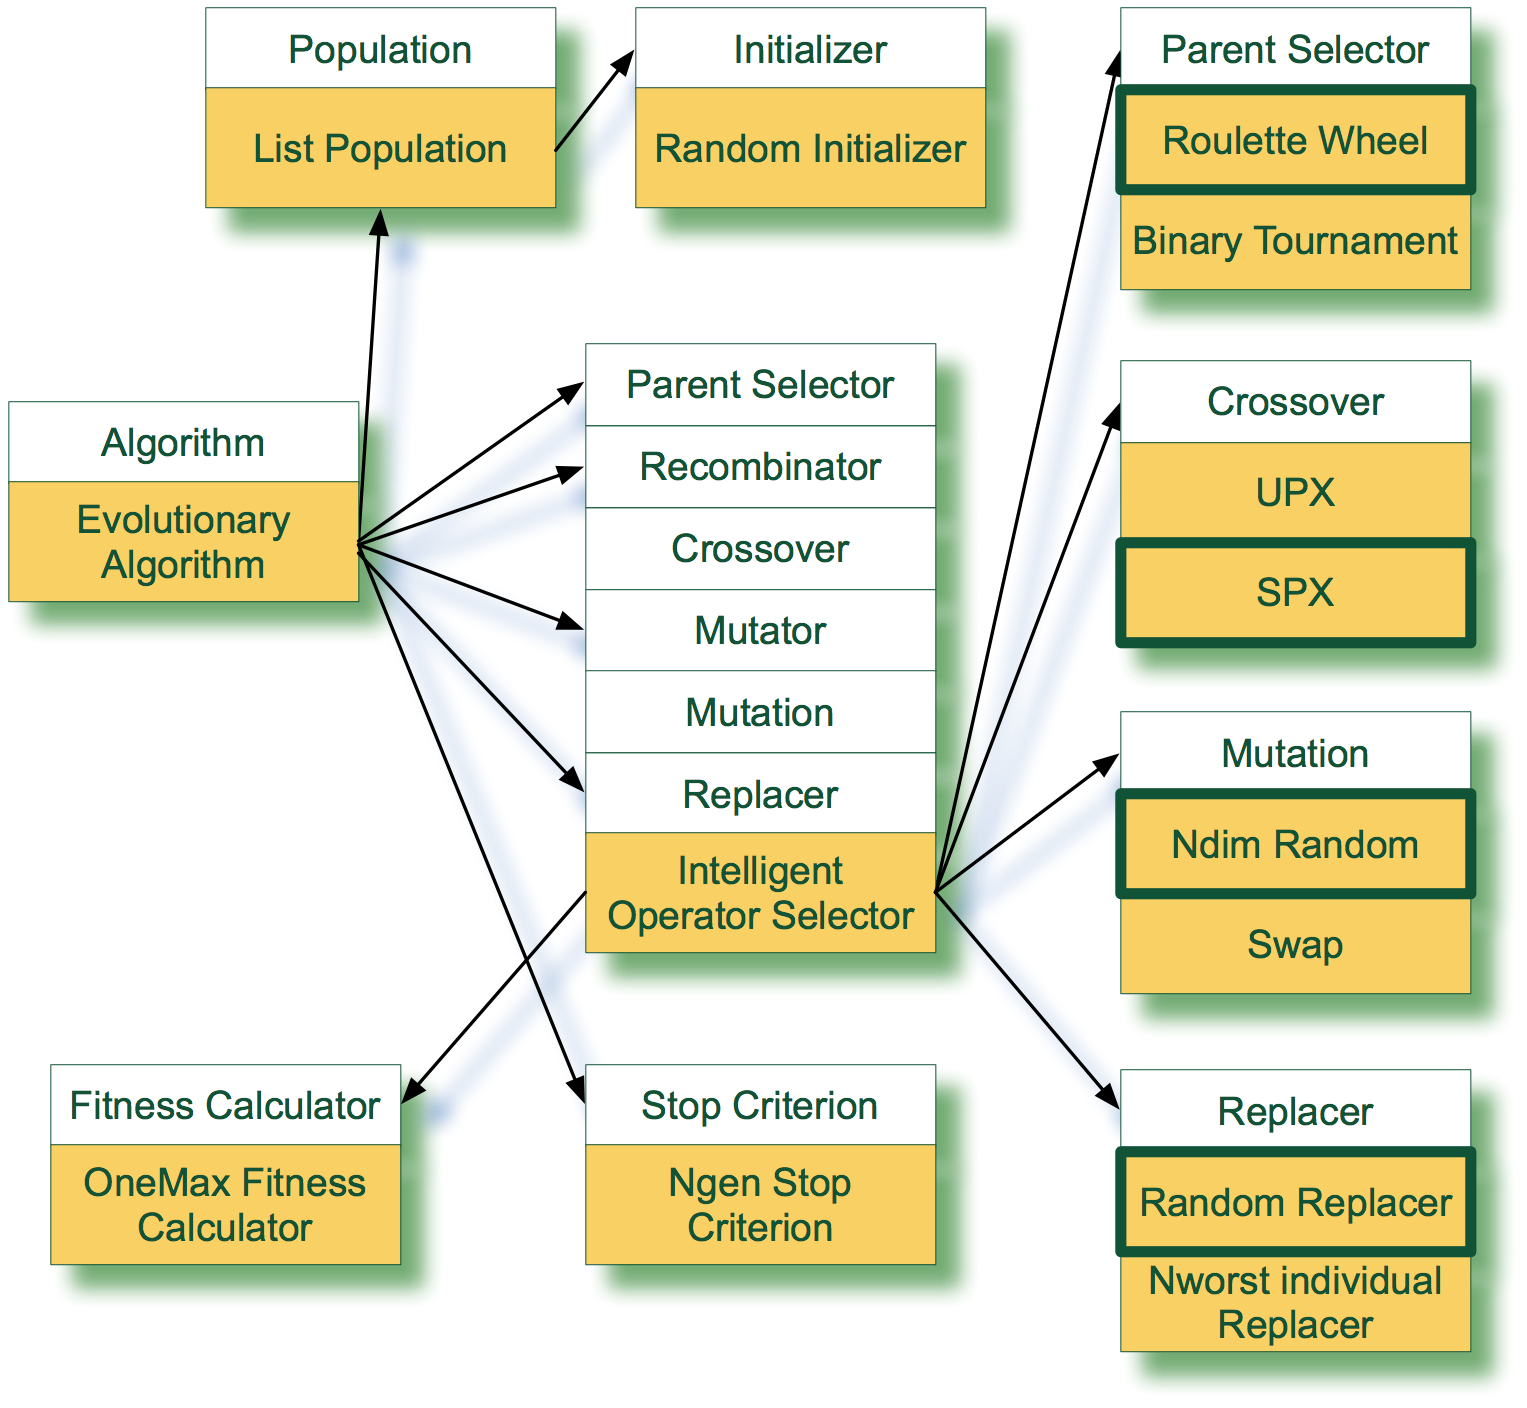
\includegraphics[width=10cm]{gfx/soaea/intelligent.jpg}
\caption{Self-adaptable Algorithm. The {\em Intelligent Operator Selector} selects which service implementation is used each time.}
\label{INTELLIGENTALGORITHM}
\end{SCfigure}


Finally, another important usage of EAs is its hybridization with other metaheuristics, to obtain more effective search algorithms \cite{HybridRodriguez2012},  increasing the performance of intensification and diversification mechanisms. With  traditional frameworks this task can be difficult, mainly because the source code for each metaheuristic must be modified. Nevertheless, using SOA a combination of loosely coupled services could be used.



The questions presented in Section \ref{subsec:soaea:implementation} have been answered to obtain the next restrictions for the desired framework. Initially, the services can be executed locally, they must be dinamically bound and no extra code should be added to allow the distribution of the created implementations. This implementation should allow asynchronous data sending/receiving, without the need to implement
  specific functions in the source code, like MPI or other
  distribution mechanisms. EAs developers can use the existing
  distribution services or create new ones, if they want. New improvements can be added
  without modifying the existing modules, that is, adding or modifying
  only the affected service implementations without modifying the
  source code of the other services.

\section{Implementation and Deployment}

\subsection{Select the technology to use}
\label{sec:osgiliath:technology}

Of the existent technologies for SOA (presented in Section \ref{chap:soa:implementations} Web Services and OSGi have been considered.
% Primero: esto debería ir al principio, incluso en la intro. Segundo
% ¡no uses items! Cuéntalo, nárralo, úsalo como argumento - JJ FERGUSON: Movido y re-escrito (muevo abajo todos tus comentarios juntos)
% ¿Faster que qué? - JJ FERGU: WS
% si no lo vas a usar en tu tesis, eso no
                            % importa nada. No añadas ruido ni razones
                            % espúreas - JJ FERGU: Evorobot
% ¿OSGi no es un
                                % servicio web?  - JJ FERGUSON: No
% Esto tienes que probarlo. No te cuesta trabajo hacer un mínimo
% servicio web para probar qué es mejor; también está el paper de
% Pedro - JJ FERGUSON: TODO
% ¿Seguro que no hay nada parecido en los servicios web? - JJ FERGUSON: 

% esto tendrías que haberlo presentado, en vez de como hechos
% consumados, como una historia. "A la hora de implementar,
% consideramos dos paradigmas diferentes (o tres). Lo que
% necesitábamos, como se dijo bla y bla, era bla y bla. Ergo elegimos
% esto porque tenía bla y bla y el otro sólo tenía bla
% No justifiques
% nada a posteriori, sino a priori, la tesis tienes que construirla,
% no justificarla - JJ FERGUSON: tienes razón, cambiado entero

OSGi has been selected because it is faster than Web Services, because it was designed for 
  lightweight devices \cite{LimGateway08}. Therefore, it can be
  used in embedded devices, like Evolutionary Robotics
  \cite{Garcia2012testing}. On the contrary, as explained in Section \ref{chap:soa:implementations} Web services were created to integrate complex
  data interchange among different companies. This is related with the transmission protocol in web services is SOAP, which implies
  the transmission of an XML ({\em eXtension Markup
    Language}) file \cite{XML}. This file is usually too large (for example, a
  complete list of workers in a company). EAs often need to send
  minimal information, but a large number of times (for example, the
  fitness of several individuals), so a complex transmission protocol
  is not recommended. OSGi includes a lot of mechanisms for data
  transmission, allowing more flexibility depending on the execution environment of
  the algorithms (for example, in a machine, in a local
  network, over the Internet, or even in more lightweight devices). 

Unlike web services, OSGi includes a blackboard event-manager,
   that is, services inform what they are doing without indicating 
 any receiver. Other services can filter this information and actuate
 accordingly, so the synchronization is easier. For example, it is not
 mandatory to create a variable to count the number of times that the
 {\em Fitness Calculator} service is executed: an external service can
 track this number. 

Other reason to use OSGi is the separation between OSGi and the source code of the
   services, so the code of OSGi-based applications can be used in other
   Java-based applications without OSGi. For the same reason,
   frameworks written in Java can be migrated into services in a easy
   way.

Finally, OSGi includes other features that, although they are not related to SOA, facilitate the service development and deployment: version and package
   control, security and life-cycle management of the used
   components, that can be useful in the development of EAs 
   (as explained by \person{Wagner \etal} \cite{WagnerPlugins07}). These advantages can be used by the EA developers if
   they work in a team collaboration. % Pero ¿lo son? - JJ

ECF\footnote{\url{http://www.eclipse.org/ecf/}} has
 been chosen because it is the most mature and accepted implementation
 (claimed by \person{Petzold \etal} \cite{petzold2011dynamic}), % o
                                % sea, que no lo has probado - JJ FERGU: no, lo ha dicho el tipo ese
and it also supports the largest number of transmission protocols,
including both synchronous and asynchronous communication. It provides
a modular implementation of the OSGi 4.2 Remote Services
standard\footnote{\url{http://www.osgi.org/Release4/Download}}. % Una
                                % vez más, NUNCA JUSTIFIQUES A
                                % POSTERIORI. Una tesis es una
                                % descripción de un camino. Quería tal
                                % cosa y tal otra cosa porque eran
                                % importantes para tal y tal
                                % cosa. Estaban tal y tal, pero cólo
                                % cual o pascual tenía lo que yo
                                % buscaba- JJ

ECF includes a number of protocols for service discovery and service providers:
\begin{itemize}
\item Service Discovery API: Includes protocols to announce and discover remote services: Zeroconf, SLP/RFC 2608, Zookeeper, file-based and others \footnote{\url{http://wiki.eclipse.org/ECF_API_Docs\#Discovery_API}}.
\item Remote Service API: Includes protocols to establish the communication (data streams, formats and others): R-OSGi, ActiveMQ/JMS, REST, SOAP, XMPP, ECF Generic \footnote{\url{http://wiki.eclipse.org/ECF_API_Docs\#Remote_Services_API}}. This allows communication with systems that do not use OSGi or Java.
\end{itemize}
% Vale. ¿y? ¿Lo vas a usar luego? - JJ FERGUSON: si, en siguientes capítulos volveré a referenciar esto

More information about the application of OSGi in other areas, with
good practices, benefits and lessons learned is provided by the
authors in \cite{GarciaSanchez2013Gateway}. 



%FERGUSON: He comentado TODO lo que venía ahora
%\section{Framework description}
% no label? - JJ
%This proposed environment is a  framework for the development of
%heuristic optimization applications, not focused on a concrete
%paradigm, and whose main objective is to promote SOA benefits % ¿dónde? - JJ
% and offer these features to programmers: % ¿Por qué? - JJ


%\begin{itemize}
%\item Well defined interfaces. As previously stated, service
%  interfaces have been designed to be as abstract as possible. %¿have
                                %been o will be? ¿Es parte de la tesis
                                %o no? ¿Lo has hecho ya en otro
                                %capítulo? - JJ
%\item Asynchronous data sending/receiving. Due to the distribution
%  capabilities offered by OSGi, the presented implementation allows
%  the direct distribution of services, without the need to implement
%  specific functions in the source code, like MPI or other
%  distribution mechanisms. EAs developers can use the existing
%  distribution services or create new ones, if they want. % En
                                % general, deja claro si esto lo has
                                % deducido tú, es necesario, es una
                                % decisión entre muchas, qué diablos
                                % es y como encaja con TU TESIS - JJ
%\item Service oriented programming. New improvements can be added
%  without modifying the existing modules, that is, adding or modifying
%  only the affected service implementations without modifying the
%  source code of the other services. %¿Esto no lo tiene OSGi de por
                                %sí? - JJ
%\item Server/client or distributed model. All the components of this
%  implementation can communicate in a bi-directional way, so it is not
%  mandatory to use a central server to manage other nodes. % ver
                                % arriba - JJ
%\item Paradigm independent. Although the first developments are focused on EAs, this architecture can be extensible to other kinds of metaheuristics.
%\item Remote event handling. Users can handle a
%  powerful synchronization tool among distributed services using OSGi
%  features.  % ein? - JJ
%\end{itemize}

%\subsection{OSGiLiath organization}

%By now, OSGiLiath counts with the next bundles: %No es un manual. Es
                                %una tesis. Cuenta por qué tiene esos
                                %bundles, qué te ha llevado a
                                %hacerlas, etc etc. ¡Una tesis es una
                                %tesis! - JJ FERGUSON: Comentado (mover a un apéndice?)


%\begin{itemize}
%\item osgiliath: This is the core bundle. It includes all the interfaces common to the algorithms such as {\em Algorithm}, {\em AlgorithmParameters} or {\em Problem}. 
%\item Evolutionary Algorithm:  Includes the {\em EvolutionaryAlgorithm} implementation and interfaces to create the rest of the services that form an EA: {\em Recombinator} and {\em Crossover}, {\em Mutator} and {\em Mutation}, {\em StopCriterion} or {\em FitnessCalculator}. It also provides interfaces for the creation of individuals: {\em Individual}, {\em Fitness}, {\em Gene}, and {\em Genome}. 
%\item Basic Evolutionary Components: Includes several implementations (the most common ones) of the previous interfaces: {\em ListPopulation}, {\em ListIndividual}, {\em DoubleFitness}, {\em NGenerationStopCriterion}, {\em BasicOrderRecombinator}, {\em UPXListCrossover} and others.
%\item Binary Problems: Includes implementation of well-known problems, such as OneMax and MMDP: {\em OneMaxFitnessCalculator}, {\em MMDPFitnessCalculator} or {\em BinaryProblemRandomInitializer}.
%\item Function Problems: Multi-dimensional optimization functions, such as Griegwank or Rastrigin are implemented in this bundle, with their associate Initializers or Fitness Calculators.
%\item NSGA2: Interfaces and implementations of services for the NSGA2 algorithm.
%\item OSGiLiART: Service implementation for the creation of Evolutionary Art: {\em ArtisticIndividual} or {\em HistogramFitnessCalculator} are examples.
%\item NoOSGi: Because OSGi allows the separation of source code with the OSGi framework capabilities, this bundle includes Java code to integrate the services without any specific technology (just using basic Object Oriented programming).
%\item IntelligentManager: An example of how the services can be bound/unbound in real-time. By now, in each step the {\em IntelligentRandomManager} selects randomly from the available Crossovers, Mutators and Replacers implementations.
%\end{itemize}

% ¿Todo esto es interesante para entender tu tesis? 99% de
% probabilidad de que la respuesta sea NO. Así que bórralo
% (posiblemente, como dije al principio, el capítulo entero) - JJ FERGU: borado




%The source code of OSGiLiath is available in
%\url{http://www.osgiliath.org} under a GNU/GPL license. This code is
%an updated version of the work published in
%\cite{GarciaSanchezDistributed2010}.  % Esto deberías justificarlo
                                % también - JJ

 
\subsection{Implementing the services}
\label{sec:osgiliath:implementing}
%Users have to define three elements to add a new service in OSGiLiath:
% NO ES UN MANUAL. "To easen the development of new evolutionary
% algorithms with OSGILIATH, the application interface has been
% designed so that... " - JJ

In OSGi, the services are formed by the next elements:

\begin{itemize}
\item {\em Service interface}. It is a Java interface. The user just needs to specify the operations that the service will perform.
\item {\em Service implementation}. The programmer just writes the code of the interface methods.
\item {\em Service description}. It is an XML file that indicates which
  interface is being implemented and which other services needs to be
  activated. 
\end{itemize}
These concepts are explained in detail in Appendix \ref{chap:appendixosgi}. % ¿Dónde? Etiqueta secciones para poder referirte a ellas - JJ FERGU: movido al apendice

In this step the interfaces of the services identified in
Section \ref{sec:soaea:creating}, such as {\em Algorithm}, {\em
  StopCriterion}, {\em Population} or {\em Recombinator} are implemented in Java. These
interfaces are grouped along other interfaces that do not need to be a
service. For example, the interface of the object {\em
  Individual}. This interface is used in the {\em Recombinator}
interface, which receives a list of {\em Individual} objects to be
recombined, and returns another list with the recombined ones. 
Also, several implementations are included, like {\em
  EvolutionaryAlgorithm} (implementing {\em  Algorithm}) or the rest
of  services explained in previous chapter, like the services for
NSGA-II. % Para que... ¡no describas, justifica! ¡¡¡¡Es una tesis!!! - JJ

Then several of these interfaces have been implemented: examples are TPXCrossover or List Population.

Once the services are implemented, the flow of execution must be . In previous chapter the usage of a Evolutionary Algorithm service implementation was proposed. The source code of the method that executes the algorithm in the class
{\em EvolutionaryAlgorithm} (implementation) is shown in Figure
\ref{fig:javaevo}. It includes methods to bind the six references
to the service implementations that are needed: Population ({\em pop}
in the code), StopCriterion, ParentSelector, Recombinator, Mutator,
and Replacer.  % Usa \sc o algún tipo especial para código - JJ 


\newsavebox{\mintedbox} %¿No hay nada para código? ¿Con colorines y demás? - JJ FERGUSON: si, con minted salen colorines
\begin{lrbox}{\mintedbox}
\begin{minipage}{10cm}
\begin{minted}[mathescape,
               linenos,
               frame=lines,
               framesep=2mm]{java}
//References to the implementations to use
Population pop;
ParentSelector parentSelector;
Recombinator recombinator;
Mutator mutator;
Replacer replacer;

//Example of the method to obtain an implementation
//of the ParentSelector interface 
//(one function per reference)
void setParentSelector(ParentSelector sel){
  this.parentSelector = sel;
  //now sel is a reference to an implementation 
        //of ParentSelector
}

//Implementation of the start() method of the 
//Algorithm interface
public void start(){
  pop.initializePopulation();
  actualIteration = 0;
  do{
    //SELECT parents
    List<Individual> parents = 
    parentSelector.select(pop);
      
    //RECOMBINE parents
    List<Individual> offspring = 
    recombinator.recombine(parents);
      
    //MUTATE offspring
    List mutatedOffspring = 
    mutator.mutate(offspring);
      
    //SELECT new population. 
    //pop is modified here
    replacer.select(pop, parents, 
    offspring, mutatedOffspring);
      
    actualIteration++;
      
  }while(!stopCriterion.hasFinished());
    
}
\end{minted}
\end{minipage}
\end{lrbox}
% Hay que tener mucho cuidado con poner código en una tesis porque hay
% gente que puede leérselo. Yo lo quitaría, pero si está, asegúrate
% que sigue todas las buenas prácticas. Por ejemplo, en vez de
% hasFinished debería llamarse "isMet" o
% "isTrue". initializePopulation es repetitivo: debería ser initialize
% simplemente. 
% Es más, estas críticas tendrían toda la razón de ser porque estás
% incluyendo el diseño del framework como parte de la tesis, así que
% deberías seguir todas las buenas prácticas que haya sobre el
% tema. Además, no está el código completo, ¿no? El this de la
% función ¿a qué se refiere? - JJ

\begin{SCfigure}[20][htb]
\usebox{\mintedbox}
\caption{Java code of the class {\em Evolutionary Algorithm}. This class implements the {\em Algorithm} interface, which defines the operation {\em start()} } 
\label{fig:javaevo} 
\end{SCfigure}


%This is the code needed by a EA, so it not necessary to modify it
%(for example, to change from a GA to an ES).  % eso es muy
                                % arriesgado. es un GA canónico, con
                                % un solo operador de mutación y de
                                % crossover, que lo hace exactamente
                                % en ese orden, no usa
                                % elitismo... Decir que no es
                                % necesario modificarlo es discutible
                                % y además no sé qué tiene que ver con
                                % TU TESIS - JJ FERGU: Quitado. En el anterior capitulo puse que era un ejemplo de flujo

\subsection{Deploying the services}

The services are deployed inside an OSGi container (such as Equinox or Felix). The container has mechanisms to list, start and stop services. To automatically bind the service implementations with the service interfaces                                
 the {\em Service Description} is used. % ¿Eso qué tiene que ver
                                % con el código de antes? - JJ FERGU: Añadida frase en medio
Each implementation of a service has an XML file indicating which interface is being implemented, and also other properties. This file is used by OSGi to automatically bind the services. The service descriptor of the EA is shown in Figure \ref{fig:ds}. This file describes that the {\em EvolutionaryAlgorithm} class is an implementation of the {\em Algorithm} interface, and that it needs implementations of the interfaces {\em Population}, {\em Mutator}, {\em ParentSelector}, {\em Replacer}, {\em StopCriterion} and {\em Recombinator} to be activated.

It should be noted that this file usually can be modified using a friendly GUI, or from an assistant in Java IDEs, such as NetBeans or Eclipse (so, users do not have to care about its XML structure). The user interface to create this file in Eclipse is shown in Figure \ref{fig:xmlgui}. The interface being implemented is set in the lower part ({\em Algorithm}). The necessary services to activate this implementation are indicated in the upper part (with the cardinality and functions to set and unset the service implementations in the implementation source code).

\newsavebox{\mintedboxDS}
\begin{lrbox}{\mintedboxDS}
\begin{minipage}{10cm}
\begin{minted}[linenos,
               fontsize=\scriptsize,
               frame=lines,
               framesep=2mm]{xml}
<?xml version="1.0" encoding="UTF-8"?>
<scr:component xmlns:scr="http://www.osgi.org/xmlns/scr/v1.1.0" enabled="false"
immediate="true" name="OsgiliathEvolutionary" >
<implementation class="es.ugr.osgiliath.evolutionary.EvolutionaryAlgorithm"/>
<service>
<provide interface="es.ugr.osgiliath.algorithms.Algorithm"/>
</service>
<reference bind="setPopulation" cardinality="1..1"
interface="es.ugr.osgiliath.evolutionary.elements.Population"
name="Population" policy="static" unbind="unsetPopulation"/>
<reference bind="setMutator" cardinality="1..1"
interface="es.ugr.osgiliath.evolutionary.elements.Mutator"
name="Mutator" policy="static" unbind="unsetMutator"/>
<reference bind="setParentSelector" cardinality="1..1"
interface="es.ugr.osgiliath.evolutionary.elements.ParentSelector"
name="ParentSelector" policy="static" target="(selectorName=nsga2)" 
unbind="unsetParentSelector"/>
<reference bind="setReplacer" cardinality="1..1"
interface="es.ugr.osgiliath.evolutionary.elements.Replacer"
name="Replacer" policy="static" target="(replacerName=nsga2)" 
unbind="unsetReplacer"/>
<reference bind="setStopCriterion" cardinality="1..1"
interface="es.ugr.osgiliath.evolutionary.elements.StopCriterion"
name="StopCriterion" policy="static" unbind="unsetStopCriterion"/>
<reference bind="setRecombinator" cardinality="1..1"
interface="es.ugr.osgiliath.evolutionary.elements.Recombinator"
name="Recombinator" policy="static" unbind="unsetRecombinator"/>
<property name="algorithmName" type="String" value="EvolutionaryAlgorithm"/>
</scr:component>
\end{minted}
\end{minipage}
\end{lrbox} % ¿En serio que merece la pena meter estos tochos? JJ

\begin{SCfigure}[20][htb]
\usebox{\mintedboxDS}
\caption{Service descriptor of the Evolutionary Algorithm implementation.  Figure \ref{fig:xmlgui} shows the friendly user interface to automatically create this file using the Eclipse program} 
\label{fig:ds} 
\end{SCfigure}

\begin{SCfigure}
\centering
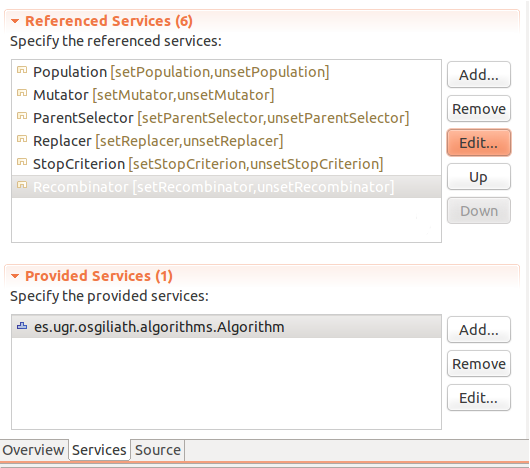
\includegraphics[width=8cm]{gfx/osgiliath/eclipse.png}

\caption{Graphic user interface in Eclipse that generates the Service Descriptor of Figure \ref{fig:ds} }.
\label{fig:xmlgui}
\end{SCfigure}



This XML file is read by the OSGi execution environment, which is the
responsible to bind the available services to this implementation. For
example, if a {\em ParentSelector} is activated, automatically is
bound to the variable {\em parentSelector} through the function {\em
  setParentSelector}. The {\em cardinality} is also set in the file,
in this case, only one implementation is necessary (not
multiple). This file can be modified in execution time, so it is not
required to re-compile the Java code to use and set new services. % zzzzzzzzz interés para la tesis: 0 - Jj

In brief, each implementation of a service (\textit{$<$im\-ple\-men\-ta\-tion$>$}) indicates the interface to being implemented (\textit{$<$pro\-vi\-de in\-ter\-fa\-ce$>$}), and the other services this implementation needs (\textit{$<$re\-fe\-ren\-ce$>$}). 

Moreover, each service can provide properties to be used by other
services to obtain more information and filtering. For example, in
this case only the {\em Replacers} whose property {\em
  replacerName=nsga2} are used. 


\subsection{Managing services: implementing the NSGA-II from the canonical GA}

Following the development example showed in Section \ref{sec:nsga2},
some extra services have been developed to convert the basic GA into a
NSGA-II %(and have also been added to OSGiLiath to be available for
%users). % ¿Lo ves como lo de arriba no incluía todos los GAs? - JJ Bueno, en teoría NO he modificado el código del EA, sólo he añadido servicios nuevos

There exist many options for the implementation of the EA to pick up the appropriate
service. % ¿El EA elige las opciones? - JJ FERGU: arreglado
 The first of them is modifying the source code of the
 implementations. Obviously this is not recommended, because the
 service would not be loosely coupled due to the specific OSGi code,
 and this is not a good SOA practice. The following ways makes the
 service usage not code-dependent: 

% No describas el ejemplo. Crea una metodología para implementar
% algoritmos y aplícala a casos particulares. Esto debería ser un
% ejemplo de una metodología más general. En la tesis no se cuenta lo
% que uno ha hecho, se cuenta la metodología que ha desarrollado uno
% para que otros puedan usarlo también. Supón guq te llega alguien y
% te dice "¿Cómo implemento un EDA?" ¿Le cuentas como se implementa
% NSGAII y que se apañe? - JJ FERGU: bueno, pues al final hice la metodología :)

\begin{itemize}
\item De-activating the implementation {\em Binary Tournament} from the OSGi administration console, and activating the implementation {\em Crowding Distance Selector} (that is, manually). This technique is not recommended, because all services are then managed by hand, and this is very difficult with a large number of services. However, the OSGi console allows modifying services in execution time, so it can be used in some cases (for example, to stop the service in a machine while another big task is being executed, and activate it again when this task is over).
\item Modifying the Service Descriptor of the {\em Evolutionary Algorithm} implementation to filter the desired implementations (for example, the attribute {\em target\-=``(selectorName\-=nsga2)''} in Figure \ref{fig:ds}). This option is used when the algorithm is fixed and does not need to be modified in execution time, and the number of operators and types are known in advance. However, as previously stated, new services can be added in execution time (for example, if the cardinality is set to multiple).
\item Using an external service that activates or de-activates desired implementations or modify their status. This technique must be used when self-adaptation properties are used in the algorithm, and it is presented in next subsections. 
\end{itemize}


None of these options needs to modify the source code of the existing
services: they just indicates which services uses each time.
% ¿Y no será más fácil tener varias implementaciones de referencia, una
% de ellas multiobjetivo como NSGAII? - JJ
% Ferguson: La cosa es elegir entre las que tienes (incluida esa)

\subsection{Making it distributed}
\label{sec:osgiliath:distributed}
% ¿Por qué no pones etiquetas de sección ? - JJ FERGU: añadida

As previously stated in the introduction of this chapter, services should be undistinguishable of being local or remote, and not to add extra code for distribution. Therefore, all services
can be distributed using the OSGi features. In this case, the
distribution is performed using the service descriptor to set which
service is distributable and which is the distribution technology that
provides service discovering and data transmission. 

As explained in Section \ref{sec:osgiliath:technology}, %¿qué sección? - JJ FERGU: Done
 OSGi allows several implementations for the service
 distribution. 
 This specification uses the OSGi service registry to expose remote services to other machines (being indistinguishable from the local ones).  ECF also separates the source code from the discovery and transmission mechanism, allowing users to apply the most adequate technology to their needs, and providing the integration with existing applications. For example, the lines of Figure \ref{fig:remote} have been added to the service descriptor of {\em MOP2 Fitness Calculator} to distribute it in the local network.

 





\newsavebox{\mintedboxServer}
\begin{lrbox}{\mintedboxServer}
\begin{minipage}{10cm}
\begin{minted}[linenos,
               fontsize=\scriptsize,
               frame=lines,
               framesep=2mm]{xml}

<property name="service.exported.interfaces" type="String" value="*"/>
<property name="service.exported.configs" type="String" 
value="ecf.generic.server"/>
<property name="ecf.exported.containerfactoryargs" type="String" 
value="ecftcp://localhost:3787/server"/>
\end{minted}
\end{minipage}
\end{lrbox}

\begin{SCfigure}[20][htb]
\usebox{\mintedboxServer}
\caption{Lines added to the service descriptor of Figure \ref{fig:ds} to be discovered by other services in a network  (this can also be done in the GUI)} 
\label{fig:remote} % Conque digas que sólo hay que añadir cuatro
                   % líneas es suficiente, no hace falta que pongas el
                   % XML - JJ
\end{SCfigure}

In this case, it is only necessary to set the properties that ECF uses
to identify the services being distributed in the network, indicating
that all implemented interfaces are distributable
(\texttt{ser\-vi\-ce\-.ex\-por\-ted\-.in\-ter\-fa\-ces}). Also, the
communication technology to be used is established
(\texttt{ecf\-.ge\-ne\-ric\-.ser\-ver}, although another kind of
protocol could be used), and finally, the service URL (\texttt{
  ecf\-.ex\-por\-ted\-.con\-tai\-ner\-fac\-to\-ry\-args}). As
previously stated, the service properties can be modified from other
services, so these properties  % THESE properties!!! - JJ
can be added outside the XML. It should be noted that the source code
of the services has not been modified to distribute them (as would
happen if MPI had been used to perform the distribution, for
example). % Pues pon como requisito desde el principio que eso es lo
          % que buscas y por eso has elegido ECF en vez de MPI o lo
          % que sea - JJ FERGUSON: añadido al principio

%\subsection{Example of programming an island model} %Sin leerlo ya te
                                %digo que lo elimines. ¿Qué quieres
                                %probar aquí? ¿Qué información añade a
                                %la tesis? FERGUSON quitado entero y reescrito en otro capítulo






%Aquí, más perdido que el barco del arroz. Todo esto parece como el
%algoritmo del tirador bizco: tiro a todos lados y acabo dando. En vez
%de hablar de implementación, tienes que hablar 
% 1. El camino que te ha llevado a usar este tipo de implementación y
% no otra y por qué has desechado los otros, incluyendo experimentos y
% referencias a "implmentation matters".
% 2. Si alguien quiere desarrollar algo nuevo, qué es lo que tiene que
% hacer. ¿Crear nuevos intelligent manager? ¿Nada? ¿Tocar las
% descripciones de servicio? 
% 3. Desarrollar, paso por paso, una implementación de algo (si puede
% ser algo que no hayas publicado todavía) y mostrar lo fácil que es,
% el poco esfuerzo necesario y las pocas líneas de código que hacen
% falta. 
% Y todo esto te lo he dicho desde el día 1. Que conste - JJ
% FERGU: reescrito todo para que cumpla los puntos




\section{Experiments} %¿Implementation o experiments? ¿Estamos a setas
% o estamos a Rolex? - JJ FERGU: Puesta frase. TERMINA
In this section, several experiments to confirm some of the advantages of using SOA and OSGi, explained in previous sections, are proposed. First, a comparison of time of using OSGi and the services as normal classes is presented to demonstrate that OSGi does not adds extra overhead (as explained in Section \ref{subsec:soa:osgi}). Experiments to demonstrate the automatic adding of new operators during runtime, and integration with other systems without modification of the existent source code are shown. Finally, a comparison of Lines of Code (LoCs) with other existent frameworks for EAs (presented in Section \ref{subsec:soaea:fworks}) is performed.

\subsection{Comparing overhead of using services}
One may think that working with services usually implies an
overhead. This is true when communication protocols like SOAP are
used, because the transmitted XML must be generated and
parsed. However, as SOA is independent of the implementations,
services also can behave as normal method calls in the same machine. 


%The first experiment of this section is focused on this issue, % ¿Qué
                                % issue? No has dicho ni qué quieres
                                % probar. Ni por qué es importante
                                % para la tesis. Ni nada. Si se trata
                                % de que OSGi no es más lento que una
                                % implementación local, tendría que
                                % haber ido al principio (y el
                                % capítulo llamarse OSGi
                                % implementation of evolutionary
                                % algorithms and its applications) - JJ
%and will demonstrate that the use of a SOA oriented % ¿a service
                                % oriented aplication oriented
                                % implmentation? - JJ
%implementation of an EA does not %nunca uses apóstrofos en lenguaje
                                %formal!!!!! - JJ
 The basic GA implemented in Section \ref{sec:osgiliath:implementing} is also executed outside of
 the OSGi framework, and a normal Java class has been used to
 integrate the interfaces and implementations ``as is''. The
 population has been set to 64 individuals, parents have been selected
 using Binary Tournament, and the mutation rate has been fixed to
 0.1. % ¿Esto influye en el resultado? Si influye, ¿has probado varios
      % settings? Si no, ¿para qué lo mencionas? - JJ FERGU: bueno, es por reproducibilidad de resultados
Worst individuals (parents and off-spring combined) are replaced, and
the stop criterion has been set to 200 generations. Each experiment
has been launched 30 times to solve the OneMax problem
\cite{SchafferOnemax91}. 

\subsection{Adding operators in runtime for self-adaptation} % ¿Una subsección? ¿Seriously? ¿Y con un párrafo? - JJ FERGU: cambiado el nombre, reescrito y movido de sitio todo lo que había

Previous sections remarked that using SOA benefits are also related
to self-adaptation. A simple example is presented here to demonstrate
how easy is to convert a basic evolutionary algorithm into a
self-adaptive one in OSGiliath. 
%In this example, an intelligent service manages all the available operators. In this case, the service {\em IntelligentRandomManager} implements the interfaces {\em Parent  Selector, Recombinator, Mutator} and {\em Replacer}. All operator implementations previously presented are added to the Manager during  runtime (see Figure \ref{INTELLIGENTALGORITHM}) when they become activated in the system. Every time the EA calls an operator, this simple manager chooses randomly one of the available implementations it controls. % ¿Eso es auto-adaptativo? Es más, para
                             % lo que haces, ¿no hay forma de hacerlo
                             % a otro nivel sin necesidad de crear un
                             % nuevo Intelligent Manager? - JJ FERGU: Borrado y puesto un experimento nuevo

                             % Me he quedado igual. ¿Ha servido esto de algo? ¿Dónde está el
% ejemplo? ¿Funciona el algoritmo mejor? - JJ FERGU: Añadido el experimento abajo, reescrito

Infrastructure services to deal with control of the population and to enable other operators are also implemented (Asynchronous Enabler Imp). Figure \ref{fig:osgiliath:enabler} shows this designed configuration.

To demonstrate that services can be managed and deployed during runtime a simple experiment is proposed. A external service to the algorithm runs in parallel consulting the population from time to time. If the best individual has not been improved in a number of times this service automatically enables another implementation of Parent Selector. This new implementation is automatically bound by the the {\em Selector Gatherer} service and start to use it. Figure \ref{fig:osgiliath:enabler} shows this configuration.

\begin{SCfigure}[20][htb]
\centering
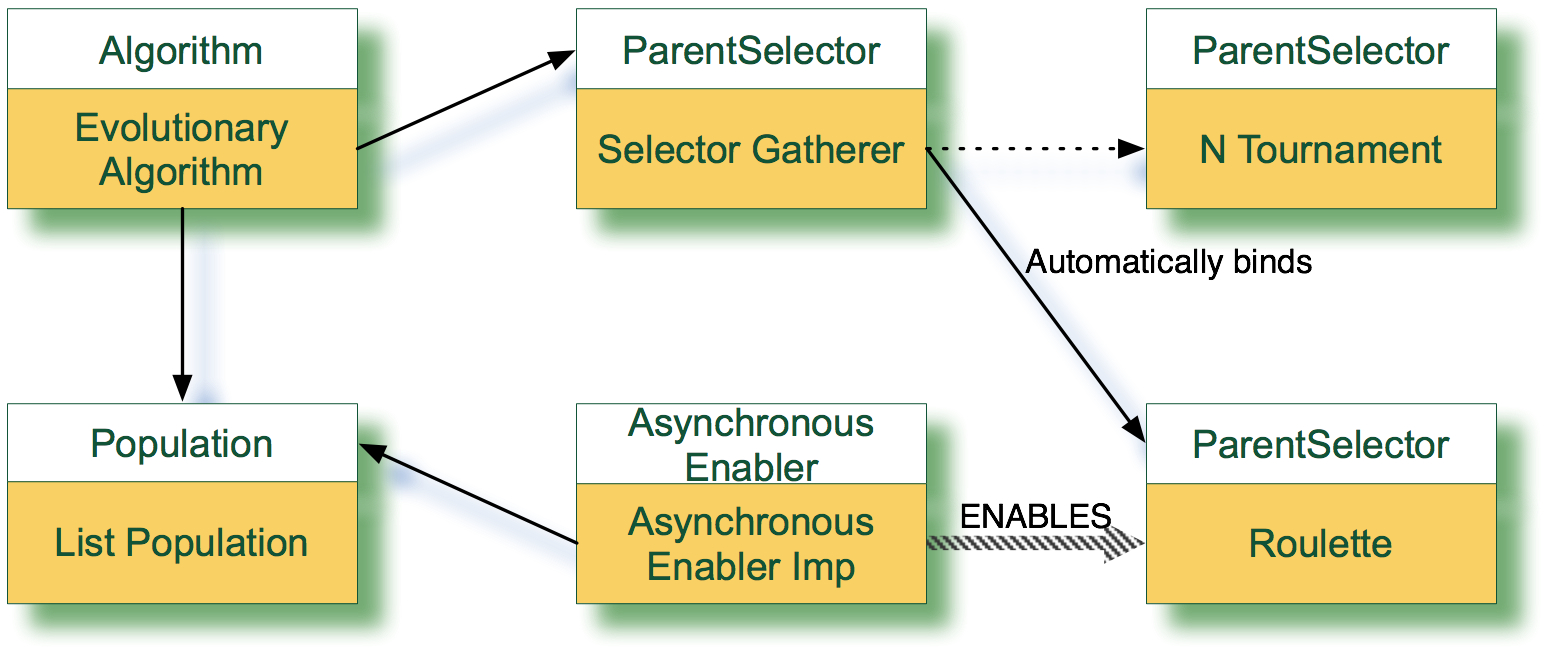
\includegraphics[width=10cm]{gfx/osgiliath/enabler.jpg}
\caption{Service that enable automatically an operator to be used during runtime.}
\label{fig:osgiliath:enabler}
\end{SCfigure}

This enabler does not affect the code of the existent services (such as Population or Evolutionary Algorithm). The gatherer also does not need specific code to acquire all
operators in execution time: it is done automatically thanks to
OSGi. In the same way as the rest of services, these operators can be activated in
execution time and added to the manager.  

This section shows the comparative results obtained using the automatic enabling of operators. Two versions have been compared: a non-adaptive version that only uses a Binary Tournament for Selection, and an adaptive one, which automatically enables a Roulette Selection when a local optimum is found. The parameters used in this comparison (accessed from the Parameters service) are a population of 64 individuals, selector rate of 0.5, TPX crossover, bit flip mutation, and individual length of 60 genes. The Roulette selector is enabled when the best individual of the population has not changed in 10 seconds (checked every 2 seconds).


\begin{SCfigure}[20][htb]
\centering
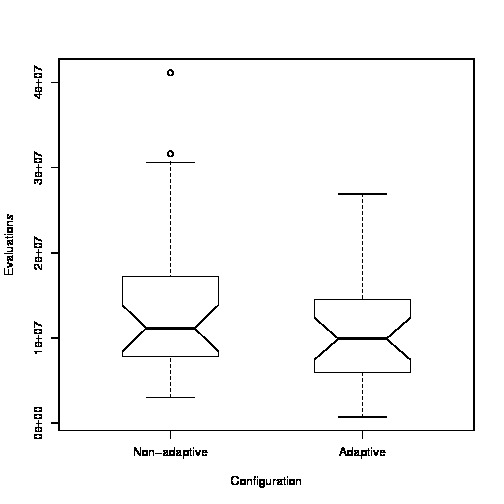
\includegraphics[width=10cm]{gfx/osgiliath/datos.jpg}
\caption{Boxplot of the number of evaluations in each configuration.}
\label{fig:osgiliath:boxplot}
\end{SCfigure}

\begin{SCtable}[][t]
\resizebox{9cm}{!}{
               \begin{tabular}{lll}
\hline

\rowcolor{colorCorporativoSuave}      & Non-adaptive & Adaptive \\ \hline \hline
\rowcolor{colorCorporativoMasSuave}Generations & 219403,10 $\pm$ 141692,16     & 167166,66 $\pm$ 93594,37 \\ \hline
\rowcolor{colorCorporativoSuave}Evaluations & 14041926,40 $\pm$ 9068298,82  & 10698794,66 $\pm$ 5990039,68 \\ \hline
\rowcolor{colorCorporativoMasSuave}Time    & 68766,40 $\pm$ 45073,04     & 51710,40 $\pm$ 29329,21 \\ \hline 
\end{tabular}
    }    
\caption{Results obtained using the Asynchronous Enabler.}
\label{tab:osgiliath:resultsenabler}
\end{SCtable}



Table \ref{tab:osgiliath:resultsenabler} shows the results obtained of the 30 executions of the two configurations tested. As it can be seen, automatic and adaptive enabling of selection operators has allowed an increase of performance, reducing time and evaluations (both significantly with a p-value$<$0.05 of a Wilcoxon test). It must be remarked that the aim of this work is not the numerical results obtained. This example has been used to demonstrate that applying a methodology to develop loose coupled services that can be dynamically bound, without modification of the existing services, can be used to achieve better results.




\subsection{Comparing with other Frameworks}
Since the OSGi framework adds features to the implementation of the
algorithm that are similar (and even superior) to those offered by
several of the frameworks described in Chapter
\ref{chap:distributedEAs}, the same algorithm (with the same operators
and parameters) has been coded using several well known frameworks, % ¿Estás comparando tu framework con el resto? Pero esto no tiene que ver con OSGi, sino con la implementación en sí. - JJ % Agh. Además, ¡¡diferentes lenguajes de programación!! - JJ FERGU: afu, fue lo que me dijeron los reviewers del paper de la SoCo, si quieres lo quito
Table \ref{tab:times} shows the execution time achieved, average
such as Mallba (C++), Algorithm::Evolutionary (Perl), and ECJ
(Java). 
solution, and Lines of Code (LoC) needed to integrate the algorithm
for each framework. All the algorithm implementations have been
executed on the same computer, an Ubuntu 12.04 Linux machine with
Intel Core2 Quad CPU Q8200 @ 2.33GHz, 4 GB RAM, without any
distribution mechanisms. The LoC have been calculated using {\em
  sloccount} program. 






\begin{SCtable}[][t]
\resizebox{11cm}{!}{
\begin{tabular}{llll}
\hline
\rowcolor{colorCorporativoSuave}Name    &  Average solution    & Average Time (s)  & LoC \\
\hline\hline
\rowcolor{colorCorporativoMasSuave}OSGiLiath               &   612.36 $\pm$ 6.05  & 0.19 $\pm$ 18.21 &  10\\
\rowcolor{colorCorporativoSuave}OSGiLiath (without OSGi)&   613.36  $\pm$ 4.50 & 0.19 $\pm$ 22.74 &  103\\
\rowcolor{colorCorporativoMasSuave}MALLBA                  &   578.76 $\pm$ 7.48  & 0.16 $\pm$ 0.0003 &  2073\\
\rowcolor{colorCorporativoSuave}ECJ                     &   602.76 $\pm$ 6.08   & 1.40 $\pm$ 0.03 &  5\\
\rowcolor{colorCorporativoMasSuave}Algorithm::Evolutionary &   617.60 $\pm$ 12.92  & 7.78 $\pm$ 0.29 &  41\\
% venga ya, 41 líneas Algorithm::Evolutionary... - JJ Fergu: Yo que se, me dio Pedro un .pl que hizo él y se lo pasé a ese
\hline
\end{tabular}
}
\caption{Comparison of tested EA frameworks in time and development.}
\label{tab:times}
\end{SCtable}

Results show that time of services of OSGiLiath is not affected by the
OSGi framework: times are almost identical to the integration with
Java code. Note that, although are services developed under SOA, and
bound in runtime, they are not distributed. Algorithmically, all
frameworks behaves the same, and results are not quite different. The
differences among frameworks are produced because the different
implementations of random generators, operators or logs, for
example. In the work of \person{Merelo \etal} \cite{PERL}, these
different behaviours are also justified. % Aquí estás comparando miles
                                % de cosas: lenguaje, máquina virtual
                                % de la misma, implementación del
                                % algoritmo, de los operadores,
                                % representación, miles de
                                % cosas. Además, es sólo 1
                                % comparación. Para ser justo,
                                % deberías comparar tamaños diferentes
                                % de cromosoma, tamaños diferentes de
                                % población y diferentes
                                % parametrizaciones. En todo caso, en
                                % una tesis con un sólo experimento no
                                % vas a ningún lado - JJ 



Regarding LoCs, MALLBA has the higher number: this is because every
% Tienes que mostrar el código y acceso a los resultados
% "crudos". Estas comparaciones de tiempo siempre son complicadas. En
% todo caso, querría ver el de A::E - JJ
algorithm is created as a ``skeleton'' and a duplication of code exist
for each algorithm and problem to execute. This is produced because
many operations affect global variables: for example the method {\em
  select\_offsprings()} affects the global variables {\em parents} or
{\em aux}. Using this method as an external service would require a
whole change in many parts of the code. Thanks the loose-coupling of
Perl, many lines of code are saved using Algorithm::Evolutionary,
mainly because many parameters and operators are defined by default. 



ECJ and OSGiLiath do not require code to combine different operators,
only to modify configuration files without re-compilation. % ¿Estas
                                % líneas las has incluido? - JJ
The difference is in ECJ the available operators must be known prior
to execution (the interfaces are linked in the source code), while in
OSGiLiath, all interfaces are bound in configuration files, or even
without them (for example, appearing in the same network/machine). But
there also exist limitations, because ECJ only provides a fixed ways
of distribution mechanisms, and only certain parts of the framework
can be accessed remotely, while in OSGiLiath all operators have the
chance to be distributed if desired, modifying the configuration
files. 


It must be remarked that OSGiLiath does not try to compete with the
other frameworks (they are widely accepted, completed and tested), it
is only an example of how to develop EAs under the SOA paradigm. % ¿Esta es la conclusión? ¿Del capítulo? FERGU: añadida sección conclusiones

\subsection{Increasing interoperability with other systems}

As previously stated, another advantage of SOA is the programming
language independence respect to the service interfaces. Although OSGi
is a kind of SOA, it does not include  the capability of
interoperability with other kind of services by default. However,
adaptation services can be added to transform OSGi interfaces into
other SOA interfaces, such as Web Services (presented in Chapter
\ref{chap:soa}). So, services that are not written in Java, neither
OSGi-based, could use services implemented in OSGiLiath (and
vice-versa). 



For example, using ECF all OSGi service interfaces are
transformed into WSDL  interfaces (explained in Section \ref{subsec:soa:ws}) automatically. % ¿Qué es wsdl? ¿Por
                                % qué es importante? ¿Lo usas? Si no,
                                % ¿por qué diablos lo dices?  JJ FERGU: referenciado, y lo uso
Thus, these services could be used from other systems, that do not
need to know the implementation language of the services in
OSGiLiath. An example where an OSGi interface is transformed into a
WSDL interface is shown in Figure \ref{AXISFIGURE}. % ¿Es tuya? ¿Por
                                % qué la pones en la tesis? - JJ FERGU: claro que es mía. La pongo porque la uso.
The computation
node A, based on OSGi, uses the OSGi interface of the computation node
C to calculate the fitness. Node B uses the WSDL interface to do the
same task. It is not necessary to modify existing services source code
to convert an OSGi interface into a WSDL interface. This
transformation is bi-directional: given an WSDL interface, it can also
be transformed into a service to use inside OSGi. For example, the
algorithms in GridUFO framework (presented in Chapter
\ref{chap:distributedEAs}) could be used from OSGiLiath. % Cada vez
                                % que dices "could be" y no "will be
                                % used and presented in Chapter A"
                                % $deity mata a un cachorro de especie
                                % en peligro de extinción de pelo
                                % sodoso y grandes ojos. - JJ






\begin{SCfigure}[20][htb]
\centering
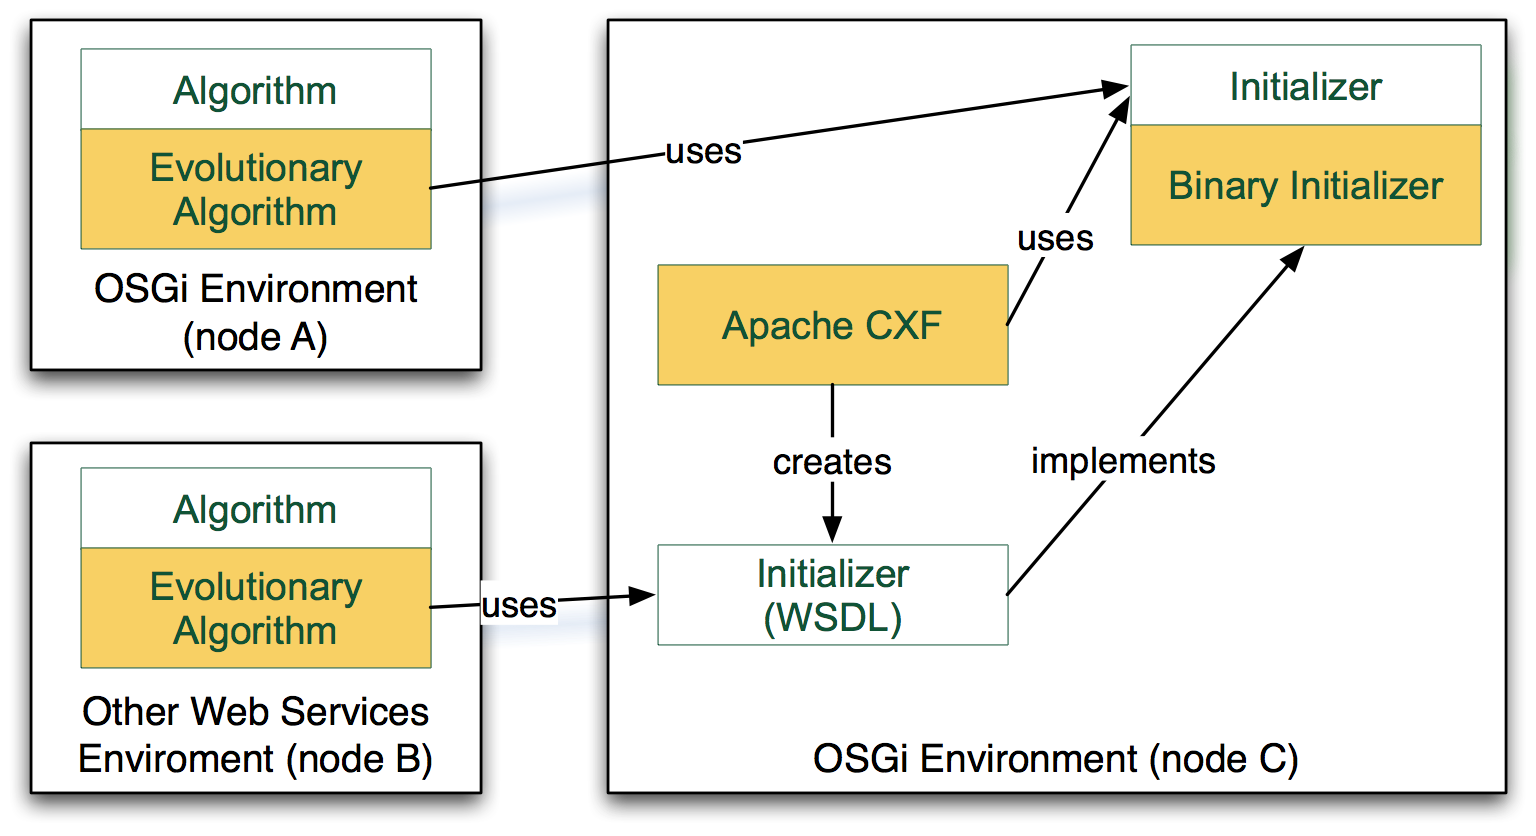
\includegraphics[width=10cm]{gfx/osgiliath/axis.png}


\caption{Communication with other kind of services. ECF service automatically creates WSDL interfaces for the OSGi interfaces to be used from other environments}
\label{AXISFIGURE}
\end{SCfigure}

\section{Conclusions}
% Tienes que alcanzar alguna conclusión fuerte: la implementación
% refleja el modelo y lo valida. ¿Es el modelo válido? ¿Cómo lo has
% probado? ¿Es la implementación válida? ¿Cómo lo has probado? - JJ FERGU: Escritas las conclusiones, que antes no había

In this chapter, the steps of implementation and deployment of services have been used to create a framework that...

The source code of OSGiLiath is available in \url{http://www.osgiliath.org} under a GNU/LGPL license.
